\documentclass[english]{article}

\usepackage{babel}
\usepackage{graphicx}
\usepackage{times}
\usepackage{pifont}
\usepackage[margin=1in]{geometry}
\usepackage{eurosym}
\usepackage{fancyhdr}
\usepackage[hidelinks]{hyperref}
\usepackage{float}
\usepackage{subfig}

\pagestyle{fancy}
\fancyhf{}


%HEADER
%**************************************************************************************
\pagestyle{fancy}
\fancyhf{}
%**************************************************************************************
\lhead{Create Database and Tables}		 	 
\rhead{Database Servers} 
\lfoot{EFA12SF}
\cfoot{\thepage}
\rfoot{Alexey Tukalo}
%**************************************************************************************

\date{}
\setlength\parindent{0pt}

\begin{document}

\title{\vspace{2in}Create Database and Tables\\
\small for Database Servers\\
\vspace{0.5in}
\includegraphics{savonia.jpg}}

\nopagebreak
\maketitle


\vspace{3in}

\author{
\begin{flushright}
Alexey Tukalo,\\
EFA12SF,\\
Information Technology,\\
Savonia University of Applied Sciences
\end{flushright}
}

\date{\today}
\thispagestyle{empty}

\newpage
\setcounter{page}{1}
\setcounter{tocdepth}{2}


%MAIN CONTENT ******************************************************************************************************************

At the start of the assignment I have created database in an according with instructions, but it was not possible to set the growth less than 500kb.
\section{Tasks 1-3}
\begin{figure}[hb]
\centerline{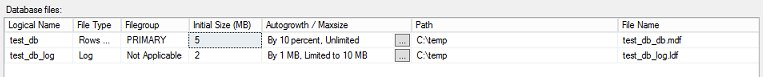
\includegraphics[scale=0.6]{SQLCreateDB/createBD}}
\caption{The database creation}
\end{figure}
The $test\_db\_new\_log.ldf$ was added with the settings from task and the size of the test\_db were increased.
\begin{figure}[hb]
\centerline{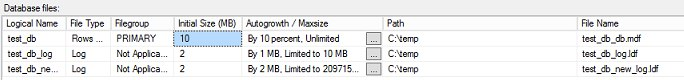
\includegraphics[scale=0.65]{SQLCreateDB/alterBD1}}
\caption{Altering of the database}
\end{figure}
\section{Task 4}
The specification is required for columns: 
\begin{itemize}
 \item emp\_no, emp\_fname, emp\_lname, (table employee)
 \item dept\_no, dept\_name, (table department)
 \item project\_no, project\_name, (project)
 \item emp\_no, project\_no. (works\_no)
\end{itemize}
It is not required for all other columns.

\begin{figure}[hb]
\centerline{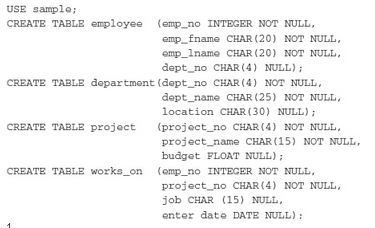
\includegraphics{SQLCreateDB/task4}}
\caption{The code from 4th task}
\end{figure}
\section{Tasks 5-11}
I have declared the customers and orders tables
\begin{figure}[hb]
\centerline{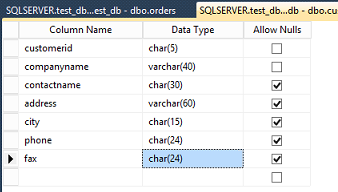
\includegraphics[scale=0.8]{SQLCreateDB/customersTable}}
\caption{Customers table}
\end{figure}
\begin{figure}[hb]
\centerline{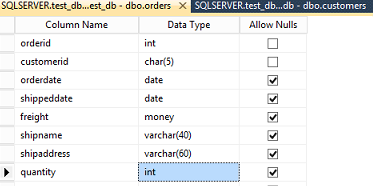
\includegraphics[scale=0.8]{SQLCreateDB/ordersTable}}
\caption{Orders table}
\end{figure}
\\And after that I altered the orders table in an according with requirements two times.
\begin{figure}[hb]
 \centerline{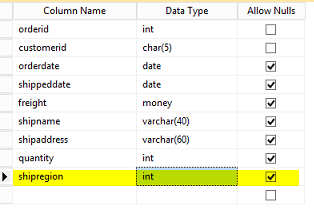
\includegraphics[scale=0.8]{SQLCreateDB/alterOrderTable}}
\caption{Alter orders table}
\end{figure}
\newpage
\begin{figure}[hb]
\centerline{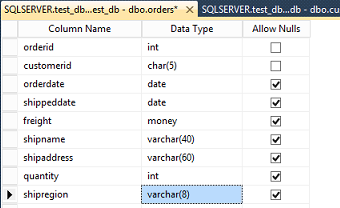
\includegraphics[scale=0.8]{SQLCreateDB/alterOrderTable2}}
\caption{Alter orders table, again}
\end{figure}
At the next step I have deleted the spipregion column and re-create tables with Primary Keys.
\begin{figure}[h!]
\centerline{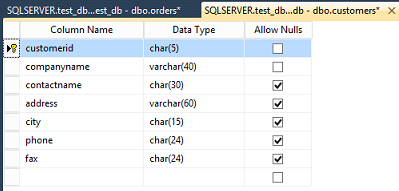
\includegraphics[scale=0.8]{SQLCreateDB/PKcustomer}}
\caption{Re-create customers}
\end{figure}

\begin{figure}[H]
\centerline{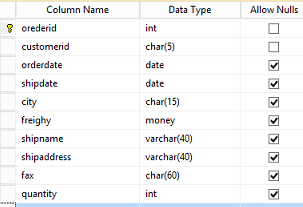
\includegraphics[scale=0.8]{SQLCreateDB/PKorder}}
\caption{Re-create orders}
\end{figure}
After an execution of the DROP TABLE statement the the information about the table would be deleted from database and the machine's memory.\\\\
The insert query is not working because the custimerid is FK and we don't have the customer with such as an id in our customers table.
\begin{figure}[H]
\centerline{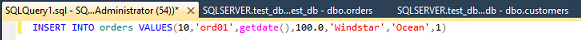
\includegraphics[scale=0.8]{SQLCreateDB/InsertWrong}}
\caption{Insert new order }
\end{figure}
\section{Task 12-15}
The code bellow allows us set current date as an orderdate in orders.
\begin{figure}[H]
\centerline{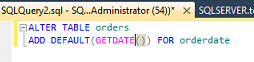
\includegraphics[scale=0.8]{SQLCreateDB/defaultDate}}
\caption{Default orderdate insert}
\end{figure}
The the source code on the picture 12 makes the value of quantity limited between 1 and 30.
\begin{figure}[H]
\centerline{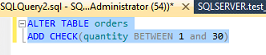
\includegraphics[scale=0.8]{SQLCreateDB/Alterquantity}}
\caption{Default orderdate insert}
\end{figure}
At the next step I have made a query to show names of the columns with int type from orders table.
\begin{figure}[H]
\centerline{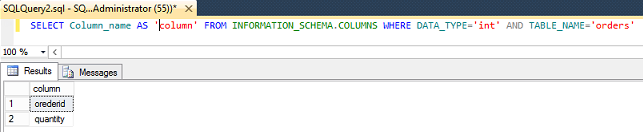
\includegraphics[scale=0.8]{SQLCreateDB/intcolumn}}
\caption{column names with int type, orders table}
\end{figure}
\section{Task 15-17}
It is not possible to delete primary key from customers table, because it makes the table an unreliable and it would also broke the reference between with orders, because it is FK for orders table, as result the database would be corrupted.
\\\\
And finally I have renamed the column city into town on the customers table.
\begin{figure}[H]
\centerline{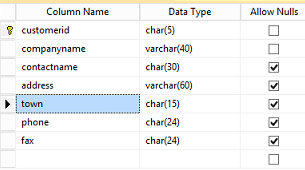
\includegraphics[scale=0.8]{SQLCreateDB/altercustomers}}
\caption{rename of city into town}
\end{figure}
\end{document}
